\documentclass[conference]{IEEEtran}
\IEEEoverridecommandlockouts
% The preceding line is only needed to identify funding in the first footnote. If that is unneeded, please comment it out.
%Template version as of 6/27/2024

\usepackage{cite}
\usepackage{amsmath,amssymb,amsfonts}
\usepackage{algorithmic}
\usepackage{graphicx}
\usepackage{textcomp}
\usepackage{xcolor}
\def\BibTeX{{\rm B\kern-.05em{\sc i\kern-.025em b}\kern-.08em
    T\kern-.1667em\lower.7ex\hbox{E}\kern-.125emX}}
\begin{document}

\title{An Evidence-Driven Fault Classification and Auto-Recovery Framework for OpenAirInterface 5G Standalone Testbeds\\
{\footnotesize \textsuperscript{*}Note: Sub-titles are not captured for https://ieeexplore.ieee.org  and
should not be used}
\thanks{Identify applicable funding agency here. If none, delete this.}
}

\author{\IEEEauthorblockN{Eueung Mulyana}
\IEEEauthorblockA{\textit{School of Electrical Engineering and Informatics} \\
\textit{Institut Teknologi Bandung}\\
Bandung, Indonesia \\
eueung@itb.ac.id}
\and
\IEEEauthorblockN{Ridha Muldina Negara}
\IEEEauthorblockA{\textit{School of Electrical Engineering} \\
\textit{Telkom University}\\
Bandung, Indonesia \\
ridhanegara@telkomuniversity.ac}
\and
\IEEEauthorblockN{Ardika Putra Hadian}
\IEEEauthorblockA{\textit{School of Electrical Engineering} \\
\textit{Telkom University}\\
Bandung, Indonesia \\
ardikaputrah@telkomuniversity.ac.id}
\and
\IEEEauthorblockN{Neil Justin Surupati}
\IEEEauthorblockA{\textit{School of Electrical Engineering} \\
\textit{Telkom University}\\
Bandung, Indonesia \\
neiljustin@telkomuniversity.ac.id}
\and
\IEEEauthorblockN{Sandrina Eka Putri}
\IEEEauthorblockA{\textit{School of Electrical Engineering} \\
\textit{Telkom University}\\
Bandung, Indonesia \\
sandrinaekaputri@telkomuniversity.ac.id}
\and
\IEEEauthorblockN{Arga Ulya Abdurohman}
\IEEEauthorblockA{\textit{School of Electrical Engineering} \\
\textit{Telkom University}\\
Bandung, Indonesia \\
argaulyaa@telkomuniversity.ac.id}
}

\maketitle

\begin{abstract}
This document is a model and instructions for aku jawa.
This and the IEEEtran.cls file define the components of your paper [title, text, heads, etc.]. *CRITICAL: Do Not Use Symbols, Special Characters, Footnotes, 
or Math in Paper Title or Abstract.
\end{abstract}

\begin{IEEEkeywords}
component, formatting, style, styling, insert.
\end{IEEEkeywords}
\section{Introduction}
\subsection{Background}
With the advent of fifth-generation (5G) mobile networks [1][2], open and flexible research platforms have become increasingly important for both academia and industry. OpenAirInterface (OAI) stands out as one of the most widely adopted open-source solutions for building and evaluating 3GPP-compliant networks, including standalone 5G (SA) deployments, Non-Public Networks (NPNs), and Open Radio Access Network (O-RAN) designs [3][4]. The complete OAI software stack enables fast prototyping independent of proprietary systems, supporting both core network and Radio Access Network (RAN) functions on commodity hardware and software-defined radio [3]. Consequently, research on network optimization, resource allocation, automation, AI-driven control, and private 5G deployment increasingly relies on OAI-based testbeds [5][6][7].
Despite their growing adoption, OAI-based 5G testbeds remain vulnerable to operational failures that jeopardize experiment reproducibility and reliability [4][8]. Common causes of failure include UE registration problems and lingering system states left behind by previous disruptions [6][9]. A major obstacle is that such failures frequently exhibit similar symptoms handling in OAI-based laboratory networks remains largely manual and highly dependent on operator expertise [10][11]. In practice, operators often prefer performing a full system restart over conducting a systematic root cause analysis. Although this action can restore the system to a functional state, the approach potentially increases recovery time, hinders the identification od the primary cause of failure, and reduces experimental reproducibility [11].

\subsection{Related Works}
\noindent 1) Open-Source 5G Testbeds and OAI-Based Deployments
Open-source platforms play a critical role in 5G research due to their flexibility and accessibility [3][5][2]. A notable example is OpenAirInterface (OAI), which has seen extensive adoption in both 4G and 5G experimentation [3][16]. Researchers have deployed 5G networks using OAI on commercial off-the-shelf hardware (COTS) paired with software-defined radio (SDR) platforms [6][4][9]. This track record reflects OAI's practically and reliability for protocol validity, performance evaluation, and experimental work spanning academic and industrial settings alike.

Throughput, latency, and signal coverage of OAI-based deployments in indoor and laboratory settings have been the subject of several prior investigations [4][8][9]. Separately, comparisons among open-source 5G testbeds under varying software configurations and deployment scenarios have also been reported [8][6]. However, most of these studies focus exclusively on testbed performance under normal, stable operating conditions; the challenges arising when testbeds experience failures remain largely unexamined [10][11]. How OAI-based deployments actually behave once failures set in, however, remains poorly documented.\\

\noindent 2) O-RAN Automation and Intelligent Network Operation
The emergence of O-RAN has spurred a substantial body of research into programmable, self-managing networks by enabling new forms of automation and intelligent control. Central to this capability is the Near-RT RIC. Combined with xApps and policy-driven control loops, it gives the network a means of responding dynamically to changing conditions, a capability that conventional RAN architectures do not offer [17][2][13].

Several testbeds built on this foundation have explored AI-driven monitoring and anomaly mitigation within O-RAN environments [7], showing that radio-access anomalies cna be detected, runtime telemetry collected, and intelligent policies applied to shape network behavior [18][12]. The bulk of this work, however, remains concentrated on radio-level conceerns and RIC-based optimization. Failures occurring deeper in the protocol, stack, such as routing inconsistencies, user-plane disruptions, tunnel failures, or lingering system states, receive comparatively little attention, even though they are frequently encountered in experimental 5G deployments [10][11].\\

\noindent 3) Reliability and Recovery in Experimental 5G Platforms
Any experimental networking platform depends fundamentally on reliability. An unstable testbed does more than interrupt ongoing experiments; it also calls into question the validity and repeatability of the results obtained. While existing deployment frameworks emphasize reproducibility through standardized scenarios and validation procedures, most of them assume that the underlying infrastructure is already operational [9][6].

In practice, however, failures do occur. When they arise in laboratory environments, recovery typically falls to experienced operators who rely on trial-and-error or full-system restarts rather than structured fault diagnosis [10][11]. Although this approach may restore the system to an operational state, it provides little insight into the actual root cause, and repeated ad hoc recovery makes experimental results harder to reproduce. Moreover, unnecessary restarts can introduce additional downstream complexity and obscure the connection between a fault and its remedy.\\

\noindent 4) Research Gap and Positioning of This Work
Based on the reviewed literature, existing studies generally fall into three groups: (i) deployment and implementation of open-source 5G platforms, (ii) deployment and implementation of open-source 5G platforms, and (iii) O-RAN automation and AI-assisted network control. Although these works have substantially advanced open-source cellular research, operational reliability management within OAI-based 5G Standalone testbeds remains largely overlooked [10][11].

Specifically, no existing work integrates fault characterization, evidence-driven diagnosis, structured recovery policies, and repeatable operational monitoring into a unified framework. Most prior studies evaluate network performance only after a successfull deployment, leaving the processes needed to detect, classify, and recover from failures largely unaddressed [4][8].

To address this gap, this paper focuses on operational reliability in an OpenAirInterface-based 5G SA/SNPN testbed. Unlike prior works centered on performance benchmarking or deployment automation, this work introduces an evidence-driven fault characterization framework, a minimal-first recovery policy, and a watchdog-assisted operational workflow, all designed to improve recovery effectiveness and experiment repeatability. Together, these contributions aim to establish a reliability layer that supports future research in AI-assisted network operation and O-RAN automation.

\subsection{Contributions and Limitations}
To adress the gaps indentified above, this paper proposes an evidence-driven operational reliability framework for OAI-based 5G Standalone Non-Public Network (SNPN) testbeds [1][3]. This framework incorporates structured health monitoring, fault characterizaito0n, evidence-based fault classification, and recovery rules that prioritize minimal intervention into a scalable operational workflow [10] [11]. Instead of triggering an immediate restart of every component, the framework instead seks out the smallest set of remedial actions sufficient to restore system functionality. Faults are classified from observable runtime indicators, including registration status, routing state, user-plane connectivity, and protocol-level signals, to guide targeted revovery [6][9]. Additionally, a watchdog-assisted monitoring mechanism continuosly records machine-readable artifacts, supporting both automated decision-making and post failure analysis [11][14].

The summarize the main contributions of this paper as follows.

1) A fault characterization framework covering common operational  failures in OAI-based 5G SA/SNPN tesbeds, including routing, user-plane, registration, and infrastructure-related fault condtions.
2) An evidence-driven, minimal-first revovery mechanism that classifies faults from observable indicators to select targeted corrective actions over blind full-system restarts.
3) A structured operational workflow integrating watchdog monitoring and machine-readable artifacts to improve experiment repeatability and operational transparency.
4) An experimental evaluation conducted on a two-node OAI 5G SA testbed, in which fault detection capability, recovery effectiveness, and operational repeatibility were assessed across a set of representative fault scenarios.\\

Experimental results demonstrate that the proposed approach reliably detects representative operational faults and restores system functionally with fewwer unnecessary recovery actions. The evidence-based recovery policy provides a practical foundation for improving the reliabiltiy of open-source 5G testbeds and servers as an enabling layer for future research in AI-assisted network operations and O-RAN automation [14][15].

\subsection{Paper Organization}

\section{Methods}
The system architecture, success-gate definition, evidence sources, fault taxonomy, recovery workflow, experimental setup, comparted methods, fault injection scenarios, procedure, sample-size rationale, and statistical analysis used in this study are presented in the following subsections.

\subsection{System Architecture}
1) OAI 5G SA/SNPN Testbed Architecture\\
An OAI-nased 5G Standalone (SA) Shared and Non-Public Network (SNPN) testbed, deployed on two laboratory virtual macines, served as the experimental platform for the work reported here. The platform was desgined to offer a controlled, repeatable environment in which operational reliablity, fault behaviour, and automated recovery in open-source 5G deployments could be examined under realistic conditions.\\
The testbed is composed of two nodes. The core node runs the OAI 5G Core Network Functions responsible for mobility management, session establishment, and user-plane services. The RAN node runs OAI gNB and UE instances, both operating in Radio Frequency Simulator (RFSim) mode so that signaling and protocol behavior can be preserved without any dependency on physical radio hardware.
\begin{figure}
    \centering
    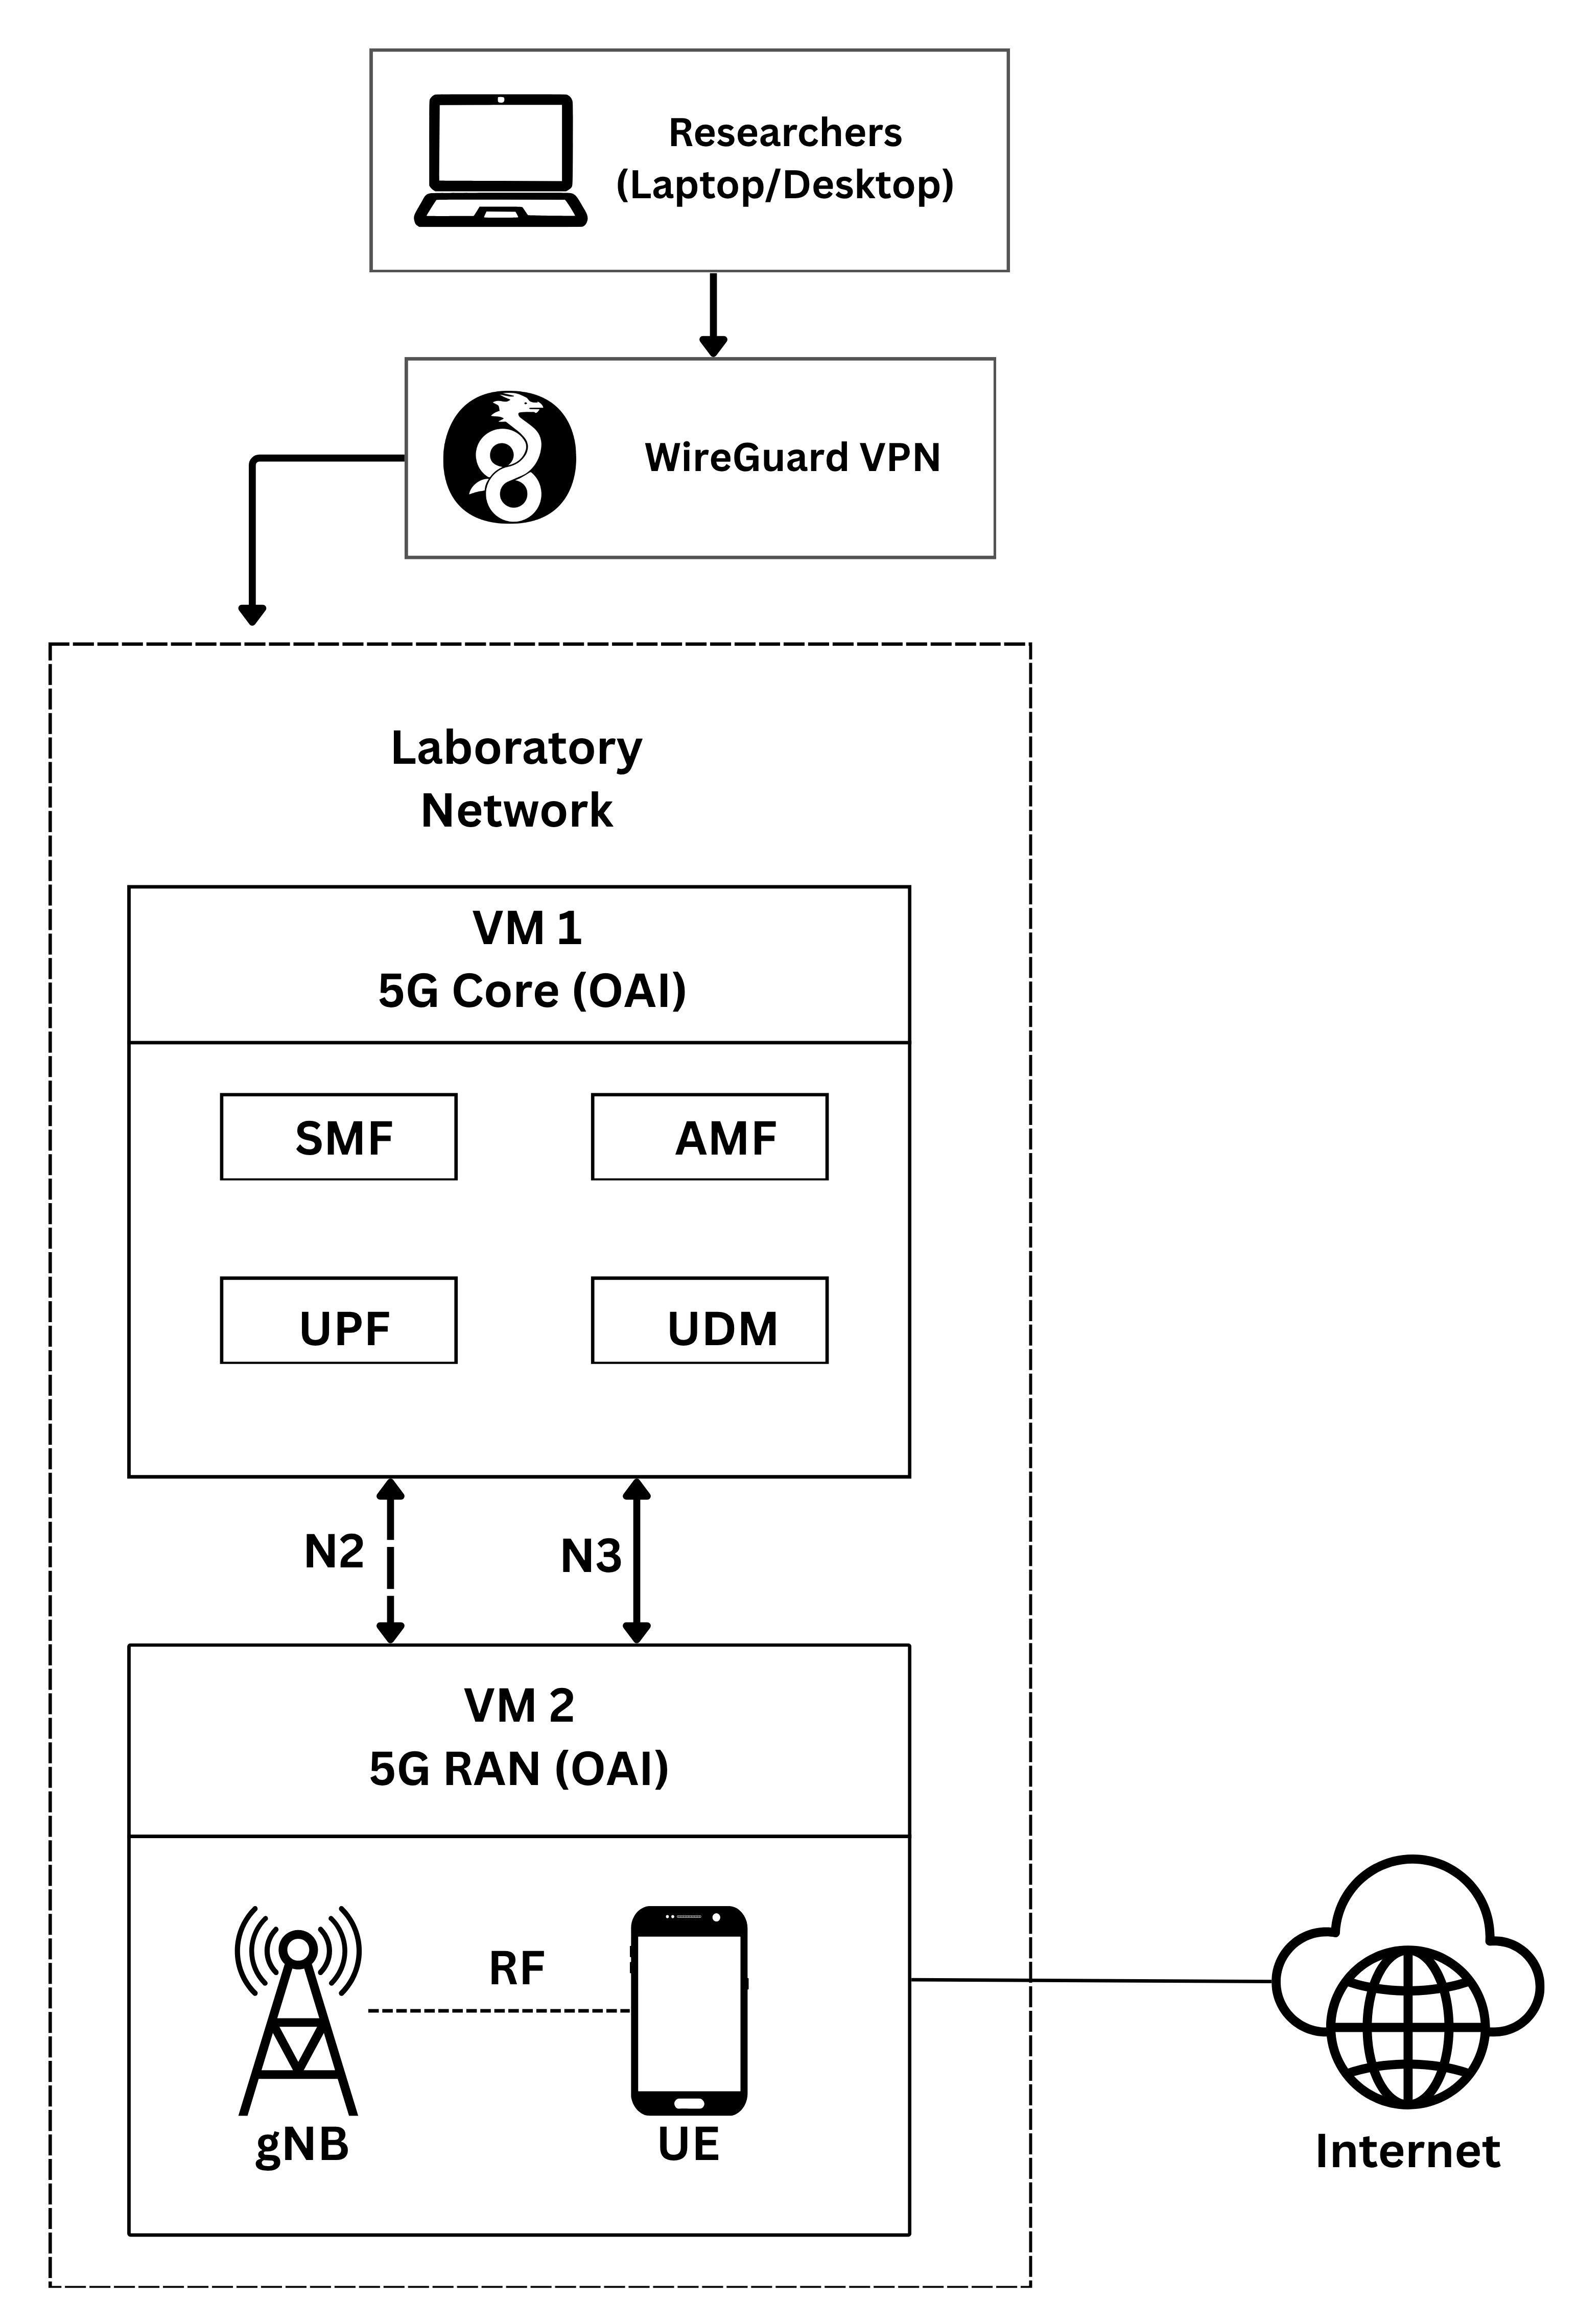
\includegraphics[width=0.7\linewidth]{Fig 1.png}
    \caption{OAI Based 5G SA/SNPN Testbed Architecture}
    \label{fig:placeholder}
\end{figure}
Interaction between the Core and the RAN follows the standard 5G Core Network functions responsible for mobility management, session establishment, and user-plane for registration and data connectivity, which keeps the environment repeatable across runs while removing the variability that physical RF conditions would otherwise introduce.\\

The testbed is reached from the local laboratory network, or remotely through a WireGuard VPN tunnel after which SSH is used to operate both virtual machines. With this configuration, monitoring, health checks, fault injection, and recovery can be carried out without anyone needing to be physically present in the laboratory, which made the volume of repeated experimentation in this study practical.

2) Success Gate and Health Indicators
Asessing whether an OAI-based 5G testbed is operational cannot be reduced to checking individual components. since a gNB can register successfully with the core while the UE still fails to obtain user-plane connectivity. A success gate was therefore introduced as a single combined criterion for testbed health, rather than relying on any one component status.

Under this definition, the testbed counts as healthy only when every gate condition holds at the same time; if even one condition fails, the state is treated as unhealthy and may trigger recovery.

Table 1. Success Gate Indicators.
The four indicators cover both control-plane and user-plane behavior. AMF association confirms that the gNB has registered with the core network. UE registration is verified by the appereance of FGS\_REGISTRATION\_ACCEPT in the UE log [19]. Tunnel avaibility checks that oaitun\_ue1 exists the correct IP configuration, and Internet reachbility checks that traffic actually passes through that pannel.

A pass on all four indicators is labeled SUCCESS\_GATE = PASS; any failure is labeled SUCCESS\_GATE = FAIL. This binary label is what the rest of the framework -- fault detection, recovery verification, watchdog monitoring -- is built around. \\

3) Evidence Sources and Fault Taxonomy 

A single log or indicator rarely tells the whole story, since different underlying faults can produce nearly identical symptoms. The diagnostic logic in this study therefore draws on several sources at once, spanning control-plane, user-plane, routing, connectivity, and process-level observations.
Table 2
A loss of internet connectivity, for instance, could stem from a routing problem, a broken tunnel, a user-plane failure, or a dead service process. Cross-checking across sources before committing to a fault label cuts down on this kind of ambiguity and avoids triggering recovery actions on incomplete information.
Faults observed during experimentation were grouped into a fixed taxonomy rather than treated as one undifferentiated category of "service down."

Table 3. Fault Taxonomy\\
Routing faults disrupt packet forwarding without necessarily touching registration. User-plane faults break data connectivity even when control-plane signalling still works. Registration faults block attachmnent outrights, and infrastructure faults trace back to a failed service or process rather than the network logic itself. 
Each fault category it tied ro a recognizable evidence pattern, derived from repeated observation during testing.


Table 4. Example Evidence-to-Fault Mapping.\\

These mappings, let the recovery engine act on a named fault category instead of a raw log output, so that each recovery decision can be traced back to spesific observable evidence rather than guesswork.

\subsection{Workflow}
\noindent 1) Operational Reliability Framework

Manual troubleshooting on a 5G testbed is slow and inconsistent, which motivated the design of an evidence-driven reliability framework that watches testbed health continuously, gather evidence when something looks wrong, classifies the likely fault, and applies a recovery action chosen from policy, targeted fixes over a blanket restart.

\begin{figure}
    \centering
    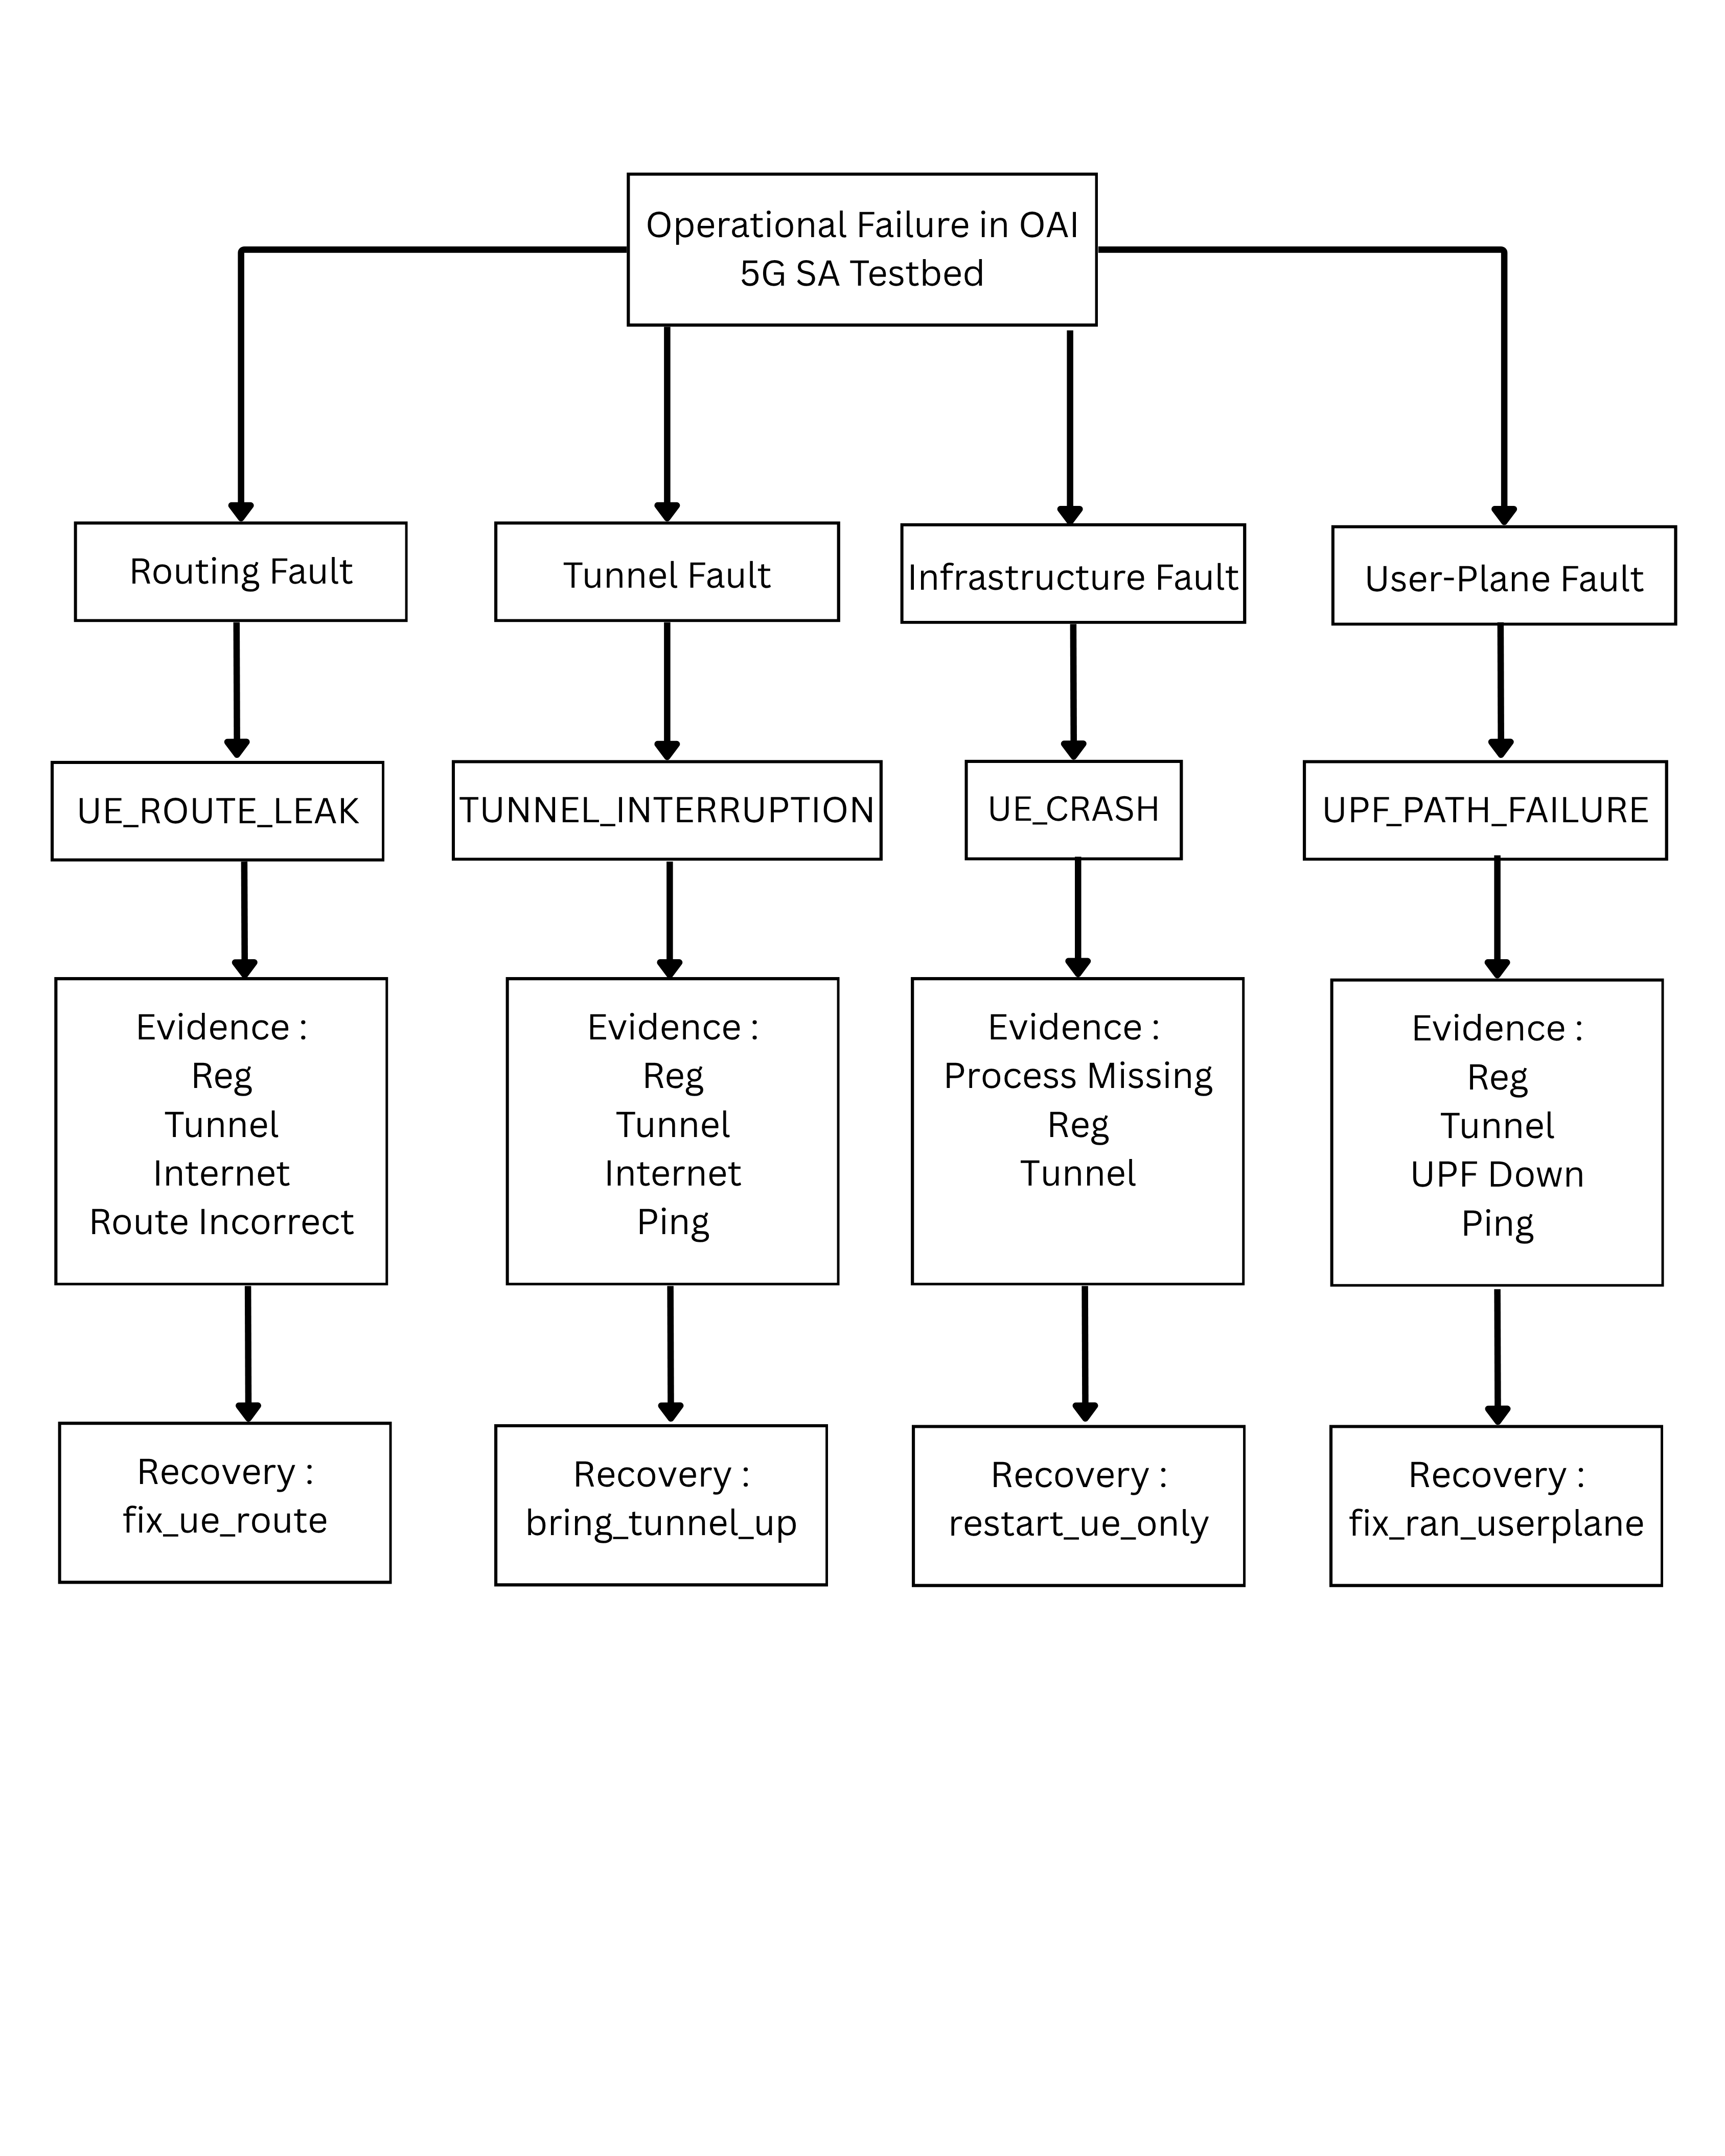
\includegraphics[width=0.8\linewidth]{Fig 2.png}
    \caption{Operational Failure Handling in OAI 5G Testbed}
    \label{fig:placeholder}
\end{figure}

Five stages make up the loop. Health monitoring runs continuously using predefined success-gate and flags degradation early. Once an anomaly appears, evidence collection pulls together registration logs, routing tables, tunnel status, connectivity tests, and process state. That evidence feeds fault classification, which maps the observed pattern onto one of the predefined fault categories instead of lumping everything under a generic failure. The recovery policy engine then picks a corrective action matched to that classification, starting from the lightest intervention and escalating only if needed. Finally, verification re-checks the success gate; if the testbed comes back healthy the loop closes, and if not, the fault is still considered active and may be escalated further.

Algorithm 1 lays out this classification and recovery logic in pseudocode. 

Algorithm 1. Evidence-Driven Fault Classification and Minimal-first Recovery.\\ \\

\noindent 2) Experimental Evaluation Setup

To test whether the framework above actually helps, its recovery behavior was compared against a blind full restart, a "kill everything and start over" approach that operational teams commonly fall back on when no fault classification is available, and one that also shows up frequently in related work. Comparing against a human operator was considered but ultimately set aside, since human response time is hard to standardize and replicate under laboratory conditions; the blind-restart baseline gives a fixed, repeatable reference point for both recovery time and action count instead. Three things were of particular interest going into the experiments: whether the classifier could reliably pin down injected faults using the available indicators (registration log, routing table, tunnel status, ping results); whether the minimal-first approach actually beat blind restart on recovery time and action count, across faults of differing severity; and whether recovery outcomes stayed consistent when the same fault scenario was repeated many times.\\

\noindent 3) Testbed Configuration

Experiments ran on the two-node testbed introduced in Section II-A1. Both nodes are virtual machines on a shared Proxmox host, with CPU and memory left uncommitted to other workloads during testing. The internal network sits on a Proxmox bridge using subnet 172.20.0.0/16; for the June 2026 experiment session, the core node was assigned 172.20.0.110 and the RAN node 172.20.0.101, with the Proxmox gateway at 172.20.0.1. Because IP assignments can shift after a reboot or topology change, addresses were re-checked before each session.

The OAI 5G Core runs on the core node as Docker containers vi   a docker-compose-basic-nrf.yaml. The gNB and UE run directly on the RAN node without containerization, using the nr-softmodem and nr-uesoftmodem binaries in -rfsim mode. The gNB configuration file (configpasti.conf) sets amf\_ip\_address to 172.20.0.110. GNB\_IPV4\_ADDRESS\_FOR\_NG\_AMF to 172.20.0.101, sdr\_addrs to "type=rfsim=, and PLMN values mcc=208, mnc=95, sst=1. The UE configuration (ue\_pasti.conf) sets -ue-nb-ant-rx- 2 -ue-nb-ant-tx 2 to meet RFSIM's radio front-end requirements.

A handful of network settings need to persist for the system to work end to end: a static route to 192.168.70.128/26 via 172.20.0.110, an iptables DNAT rule for 192.168.70.134:2152, a UDP 2152 checksum fill, PREROUTING NOTRACK, and FORWARD ACCEPT. Because VM reboots wipe out epheremal iptables rules and routes, these are reapplied automatically every 15 seconds through a system times on each node, namely oai-ran-netfix.timer on the RAN side and oai-core-netfix on the core side.

In line in the definitoin in Section II-A2, a run is treated as healthy only when all four condition hold together: the gNB is associated with the AMF over N2; the UE has received FGS\_REGISTRATION\_ACCEPT; the tunnel interface oaitun\_ue1 exists with a valid address in 12.1.1.0/24; and four-packet ICMP ping over oaitun\_ue1 to an external host (8.8.8.8) comes back with 0\% loss. This four-part gate served as the ground truth for every run [19].\\

\noindent 4) Compared Methods

Two recovery methods were tested under matching fault conditions. M\_blind, the blind full restart, runs a fixed sequence no matter what fault was injected: kill all gNB and UE processes (killall -9 nr-softmodem nr-uesoftmodem), clear the tunnel interface if it still exists, restart the gNB and wait 25 seconds for it to associate with the AMF, restart the UE and wait 30 seconds for FGS\_REGISTRATION\_ACCEPT plus tunnel re-establishment, then confirm connectivity with a ping. It reads no diagnostic evidence at any point. Instead, the same sequence, timing, and number of recovery actions are applied regardless of the fault type, making it a deterministic baseline. The script is bin/control/blind\_restart.sh.

M\_minimal, the evidence-driven method, follows the proposed evidence-driven logic. Before doing anything corrective, it gathers tunnel interface status (ip addr show oaitun\_ue1), the routing entry toward the external host (ip route get 8.8.8.8), ping results on both the default route and tunnel path, gNB/UE process status, and the AMF association count from the gNB log. The resulting pattern is matched against the defined fault categories, and the smallest viable corrective action is pulled from the evidence-to-fault mapping. For example, a routing device of eth0 with the tunnel still intact maps to 'fix\_ue\_route' (one action about 7~s); a tunnel interface in DOWN state maps to 'bring\_tunnel\_up' (one action, about 2~); an absent UE process maps to 'restart\_ue\_only' (one action about 25~s). When the evidence does not clearly point to one category, the method escalates to 'fix\_ran\_userplane'. This script is 'bin/control/autoheal\_minimal.sh'.

\begin{figure}
    \centering
    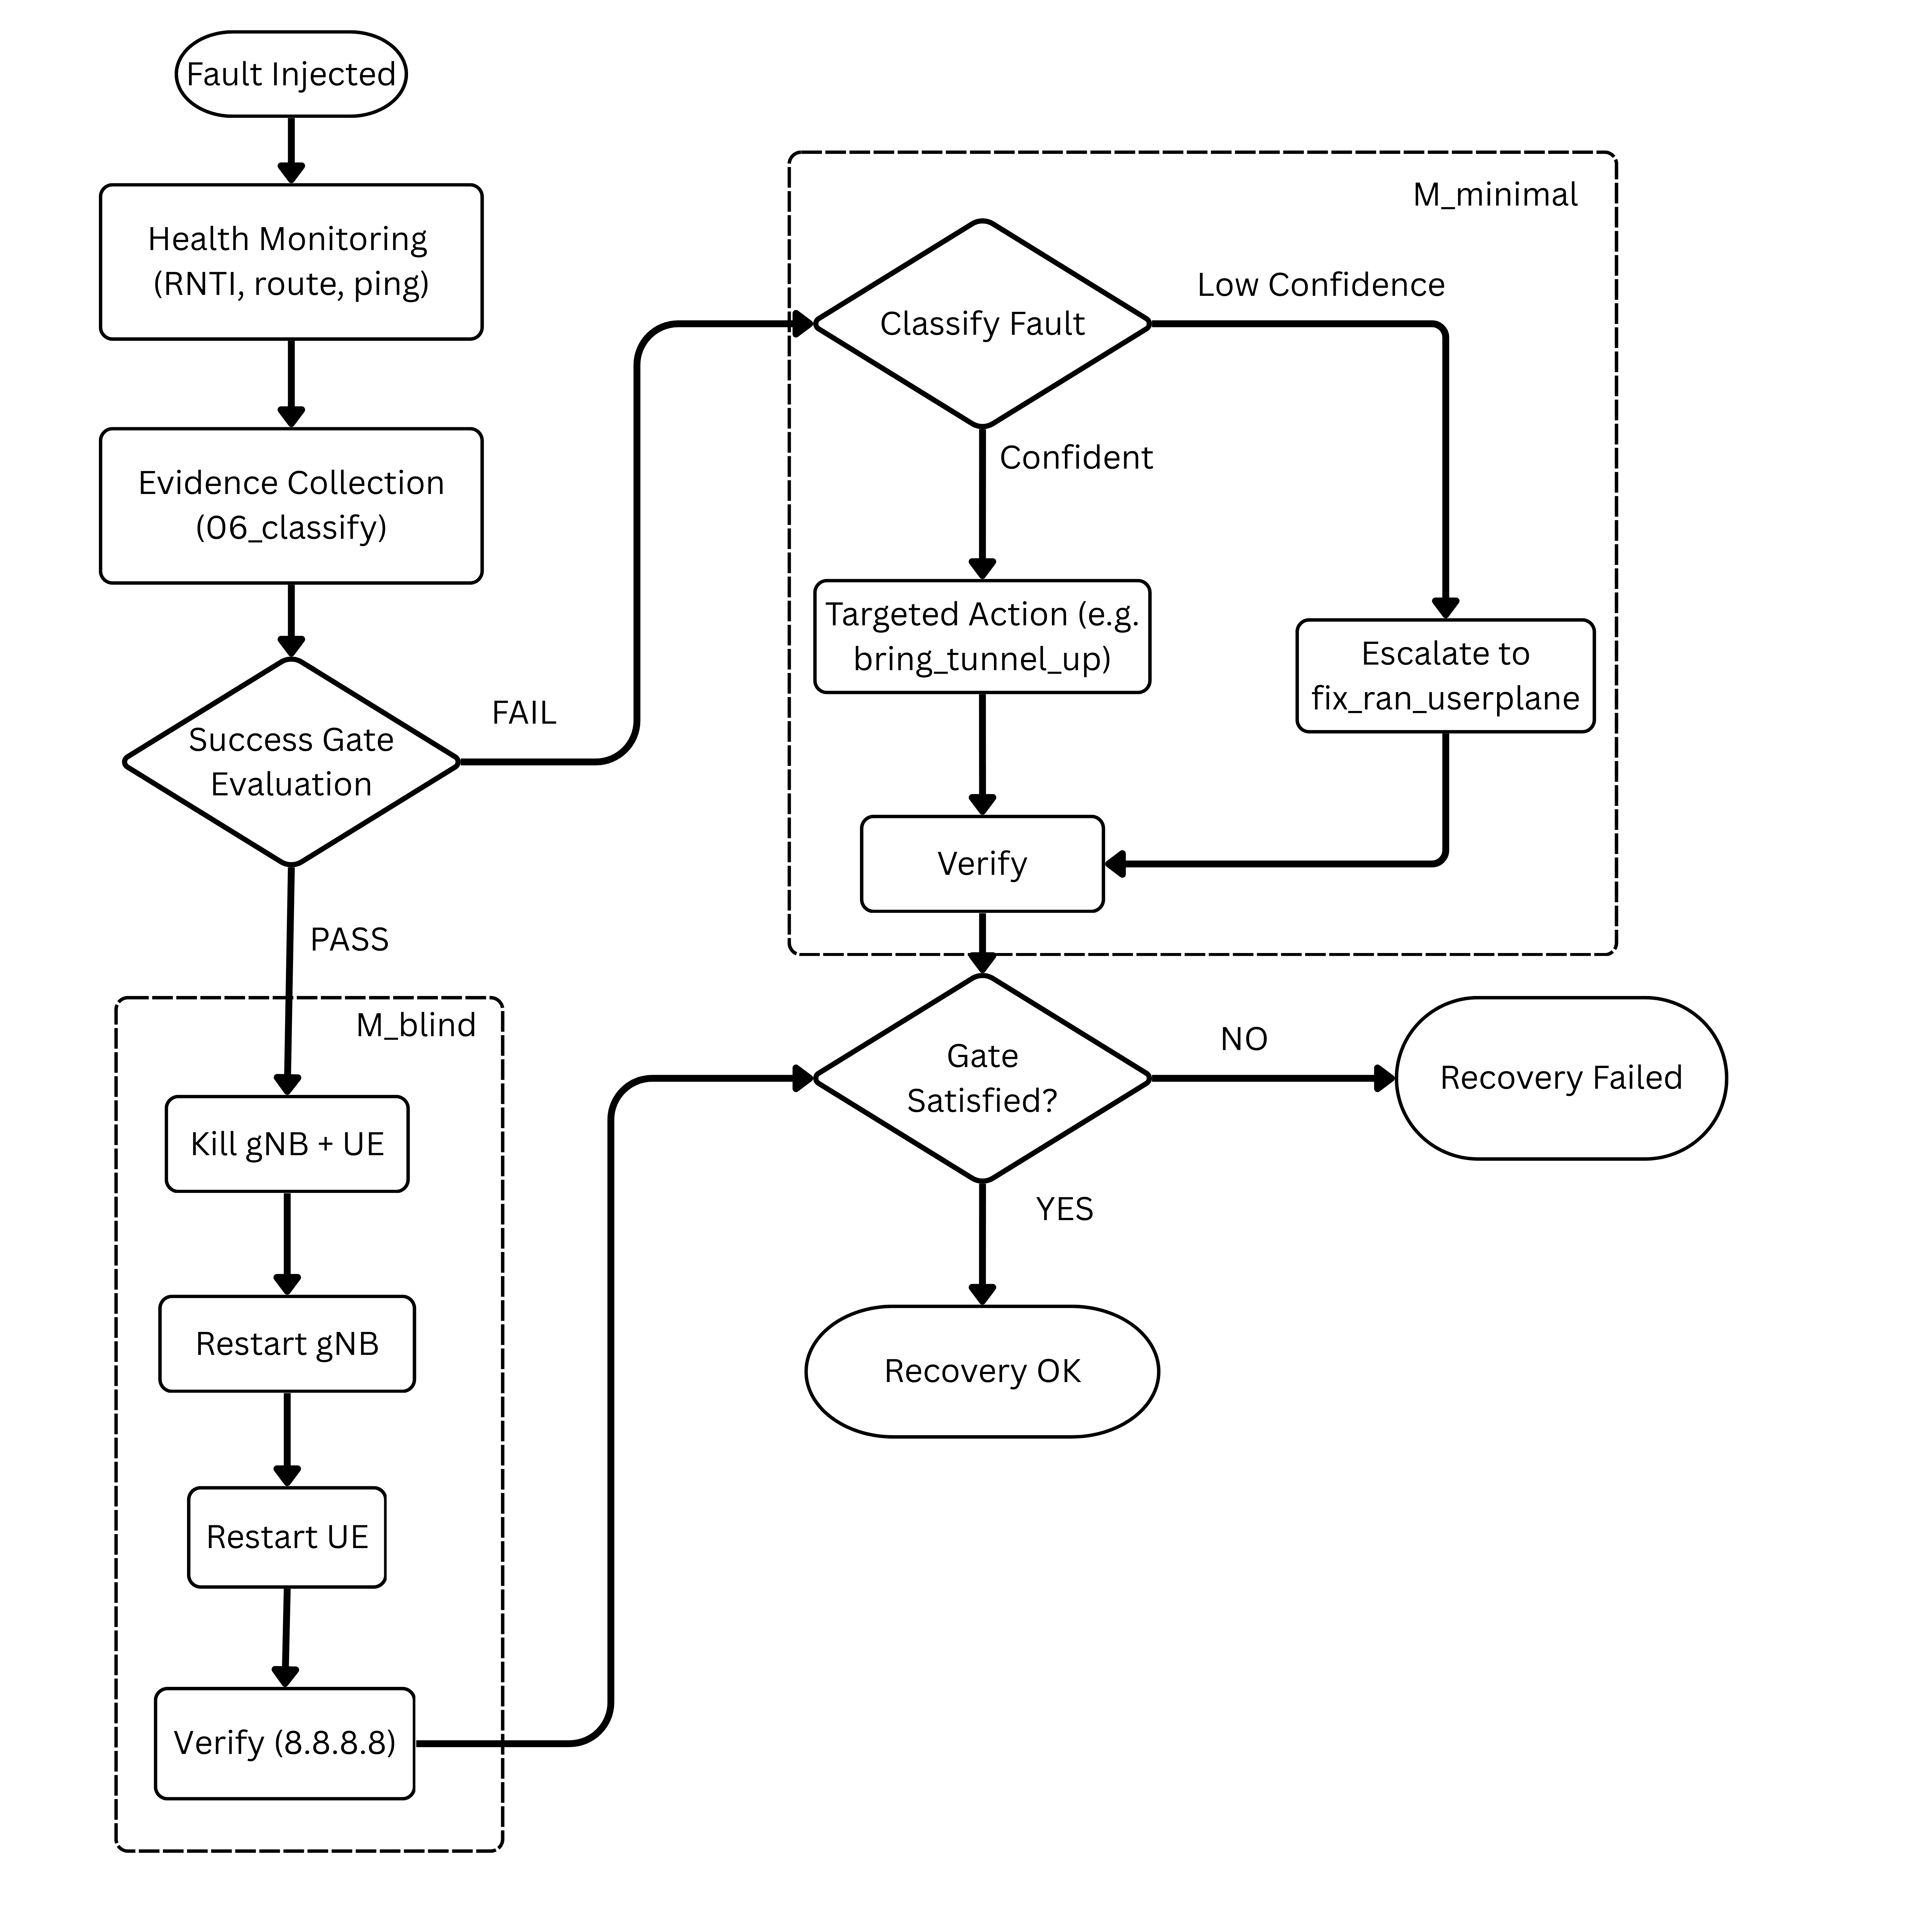
\includegraphics[width=0.5\linewidth]{Fig 3.png}
    \caption{Recovery Decision Workflow for M\_blind and M\_minimal Methods}
    \label{fig:placeholder}
\end{figure}

Both methods are wrapped as shell scripts that take '<fault\_type>' and '<run\_id>' as arguments, which lets the experiment launcher run through all 275 runs without manual intervention. Each run writes a 'summary.json' containing 'run\_id', 'method', 'fault\_type', 'recovery\_time\_sec', 'actions\_count', 'actions\_taken', 'success', and 'ue\_ip'. This fixed schema simplifies cross-method and cross-fault aggregation during the subsequent analysis.

\noindent 5) Fault Scenarios and Injection

Four scenarios were chosen from the taxonomy in Section II-A3, one from each of the routing, tunnel, infrastructure, and user-plane categories. Selection followed two rules: the fault had to be injectable and reversible without manual intervention, and its expected fix had to differ meaningfully from a blind restart. Otherwise, the comparison between the two methods would provide limit insights

Table 5. Fault Injection Scenarios.

The baseline restoration timer was paused before each injection and resumed only after recovery had completed. Otherwise, it would have automatically reversed the injected fault during the measurement, thereby skewing the recorded recovery times.

Each injection was confirmed effective before any recovery step began: UE\_ROUTE\_LEAK by checking that 'ip route get 8.8.8.8' reports eth0 as the device; TUNNEL\_INTERRUPTION by confirming the interface state is DOWN; UE\_CRASH by confirming 'pgrep -x nr-uesoftmodem' returns nothing; UPF\_PATH\_FAILURE by confirming 'ip route | grep 192.168' returns nothing. Runs where the fault could not be confirmed were flagged, pulled form the main analysis, and reported on their own.

\noindent 6) Experimental Procedure and Sample Size

Every run followed the same ten steps: confirm a healthy baseline through the success gate; pause the restoration timer on both nodes; inject the target fault per Table 5; wait 3 seconds for it to settle; confirm the fault took effect; run the assigned recovery method and time it from the first recovery action to a successful ping; re-check the success gate to confirm full recovery; resume the restoration timer; wait another 3 seconds before moving on; and write the 'summary.json' plus pre-step artifact logs.
A single M\_minimal run took 5-15 seconds depending on which action fired, while M\_blind consistently took 75-80 seconds, most of it spent waiting through the mandatory 25-second gNB restart and 30-second UE registration windows.
The full dataset combines two batches: Batch 160 (n=160, runs.csv) and a rerun, Batch 161 (n=115, runs\_rerun.csv), for 275 in total. The original plan claled for 20 runs per cell (4 faults x 2 methods) [20], or 160 runs overall; the rerun added another 115 to firm up per-cell stability, leaivng 27-41 successful runs in each cell, which is comfortably above the n=21 per-group thershold needed for Mann-Whitneyy testing at $\alpha$ = 0.05 with a moderate effect size (Cohen's $\approx$ 0.8) [21][22]. Because the two methods ended different sample sizes (M\_blind n=130,M\_minimal n=145), a balanced subsample of 260 runs (130 per method, seed=42) was also drawn by randomly dropping 15 M\_minimal runs, including three each from TUNNEL\_INTERRUPTION, UE\_ROUTE\_LEAK, and UPF\_PATH\_FAILURE, and six from UE\_CRASH. The main results below use the full 275-run dataset throughput; the balanced subsample is reported separately, purely as a robustness check. Running all 275 trials took roughly 5-6 hours of walk-clock time in total.

Runs were executed one after another rather than in parallel, since both methods touch shared testbed state: routing entries, iptables rules, and running processes. Running them concurrently would have required isolation infrastructure that the target deployment does not actually have. Statistical comparisons udes the Mann-Whitney Utest eith Bonferroni correction (adjust $\alpha$ = 0.0125 across the four faults) and Cliff's delta as the effect-size measure; success-rate comparisons used Fisher's exact test [21].

\noindent 7) Performance Metrics and Statistical Analysis

Three metrics anchor the evaluation: recovery time, success rate, and action count. Recovery time is the gap between starting recovery and reaching a healthy state again:

\begin{equation}
    t_\text{recovery} = t_\text{healthy} - t_{\text{recovery,start}}
    \label{rq:recovery_time}
\end{equation}

where $t_{\text{recovery,start}}$ marks the first recovery action and $t_{\text{healthy}}$ marks the point at which every success-gate condition is met. Success rate is simply:

\begin{equation}
    SR = \frac{N_\text{success}}{N_\text{total}} \times 100\%
    \label{eq:success_rate}
\end{equation}

with $N_{\text{success}}$ the number of runs that recovered and $N_{\text{total}}$ the total number attempted. Average recovery time and average action count per method are:

\begin{equation}
    \bar{T}_m = \frac{1}{n}\sum_{i=1}^{n} t_i, \qquad
    \bar{A}_m = \frac{1}{n}\sum_{i=1}^{n} a_i
    \label{eq:means}
\end{equation}

where $n$ is the number of repetitions and $a_i$ the action count for run $i$. The speedup of $M_\text{minimal}$ over $M_\text{blind}$ is expressed as:

\begin{equation}
    S = \frac{\bar{T}_\text{blind}}{\bar{T}_\text{minimal}}
    \label{eq:speedup}
\end{equation}

Since recovery times are unlikely to be normally distributed, significance was tested with the Mann-Whitney U statistic:

\begin{equation}
    U = n_1 n_2 + \frac{n_1(n_1+1)}{2} - R_1
    \label{eq:mannwhitney}
\end{equation}

where $n_1$, $n_2$ are the two sample sizes and $R_1$ is the rank sum of the first sample. Effect size came from Cliff's Delta, defined in terms of the sign function

\begin{equation}
    \text{sgn}(x) = \begin{cases} +1, & x > 0 \\ 0, & x = 0 \\ -1, & x < 0 \end{cases}
    \label{eq:sign}
\end{equation}

\noindent as

\begin{equation}
    \delta = \frac{1}{n_1 n_2}\sum_{i=1}^{n_1}\sum_{j=1}^{n_2}\text{sgn}(x_i - y_j)
    \label{eq:cliffs}
\end{equation}

where $\text{sgn}(\cdot)$ is the sign function defined in (\ref{rq:sign}). Together these numbers capture how effective, efficient, and repeatable the recovery process actually was across fault scenarios.

The evaluation results, including recovery-time distributions, success rate, action counts, and the corresponding statistical analysis, are presented in Section~III.

\section{Result And Discussion}

Three aspects of the proposed framework are examined here: how reliably the fault classifier identifies injected failures, how the two recovery methods compare against each other in terms of success rate, recovery time, and action count, and whether recovery outcomes stay stable when the same fault scenario is repeated.

\subsection{Fault Classification Accuracy}

\begin{figure}
     \centering
     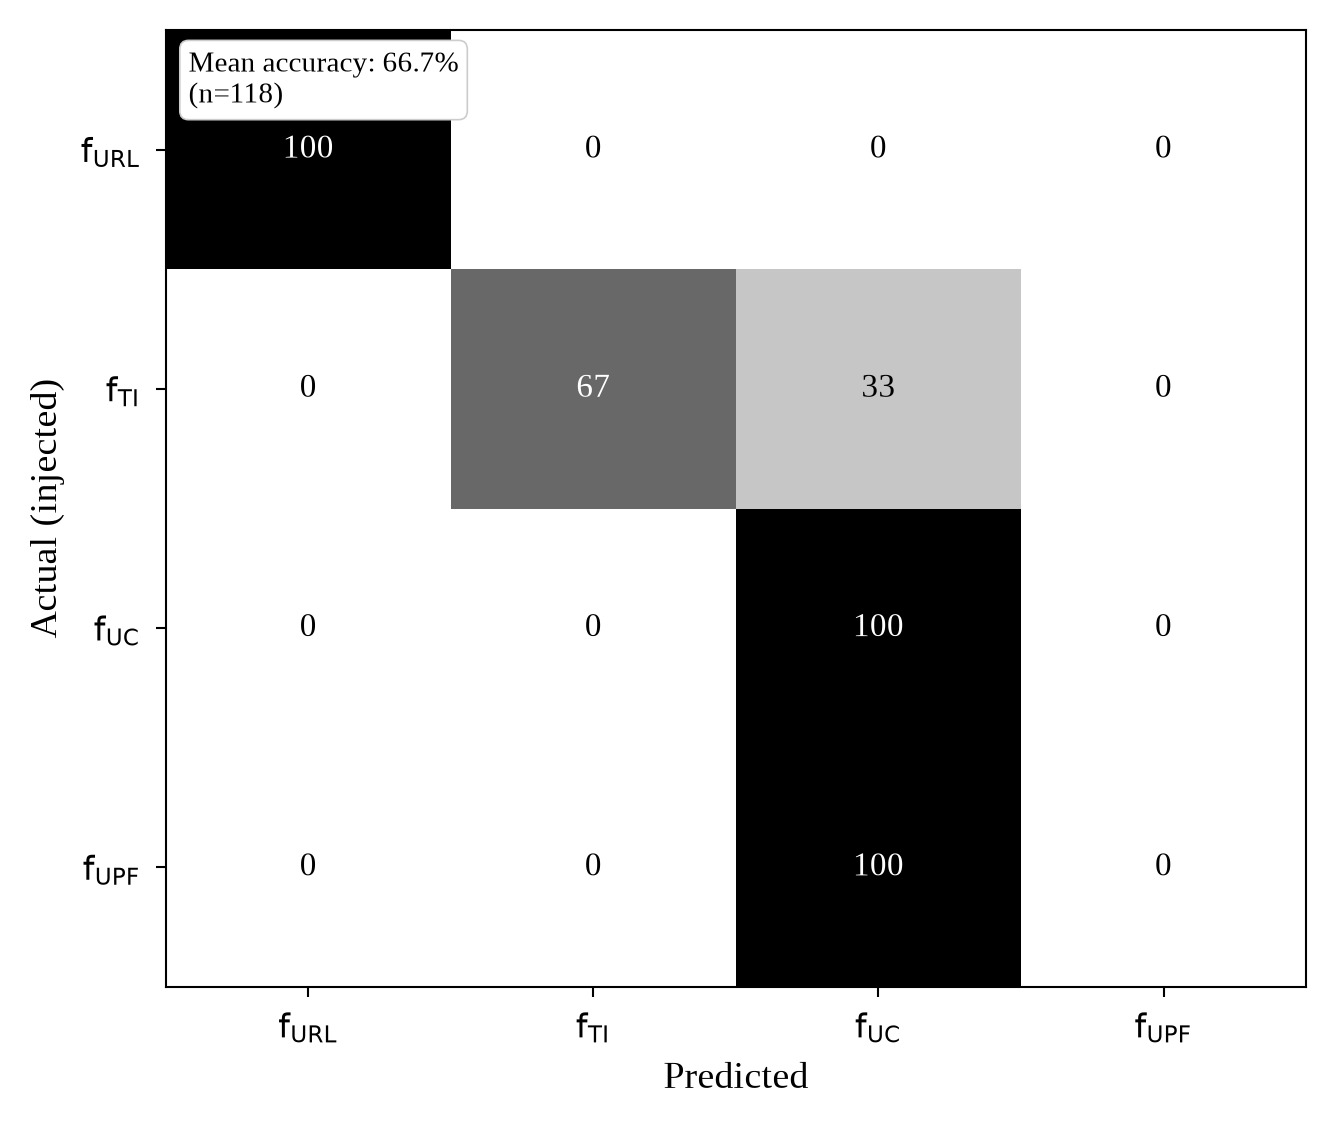
\includegraphics[width=0.5\linewidth]{Fig 4.jpeg}
     \caption{Fault Classification Confusion Matrix (n=16)}
     \label{fig:placeholder}
 \end{figure}

\text{UE\_ROUTE\_LEAK} and \text{UE\_CRASH} are both classified with perfect accuracy (100\% each). \text{TUNNEL\_INTERRUPTION} is partly mistaken for \text{UE\_CRASH} (33.3\%), and \text{UP\_PATH\_FAILURE}proves the hardest case, with all instances being labeled as \text{UE\_CRASH} (100\%). The macro-averaged per-class accuracy reaches 66.7\%, while the overall (micro/weighted) accuracy is 87.5\%, both computed across 16 held-out classified runs. The classifier therefore picks out most fault categories correctly, with confusion concentrated mainly between the use-plane and tunnel-related fault types.

\subsection{Recovery Success Rate Comparison}
This part of the evaluation checks whether M\_minimal matches or exceeds the success rate of M\_blind and M\_minimal across all four fault types, with the 90
5 target threshold indicated for reference.

\begin{figure}
   \centering
    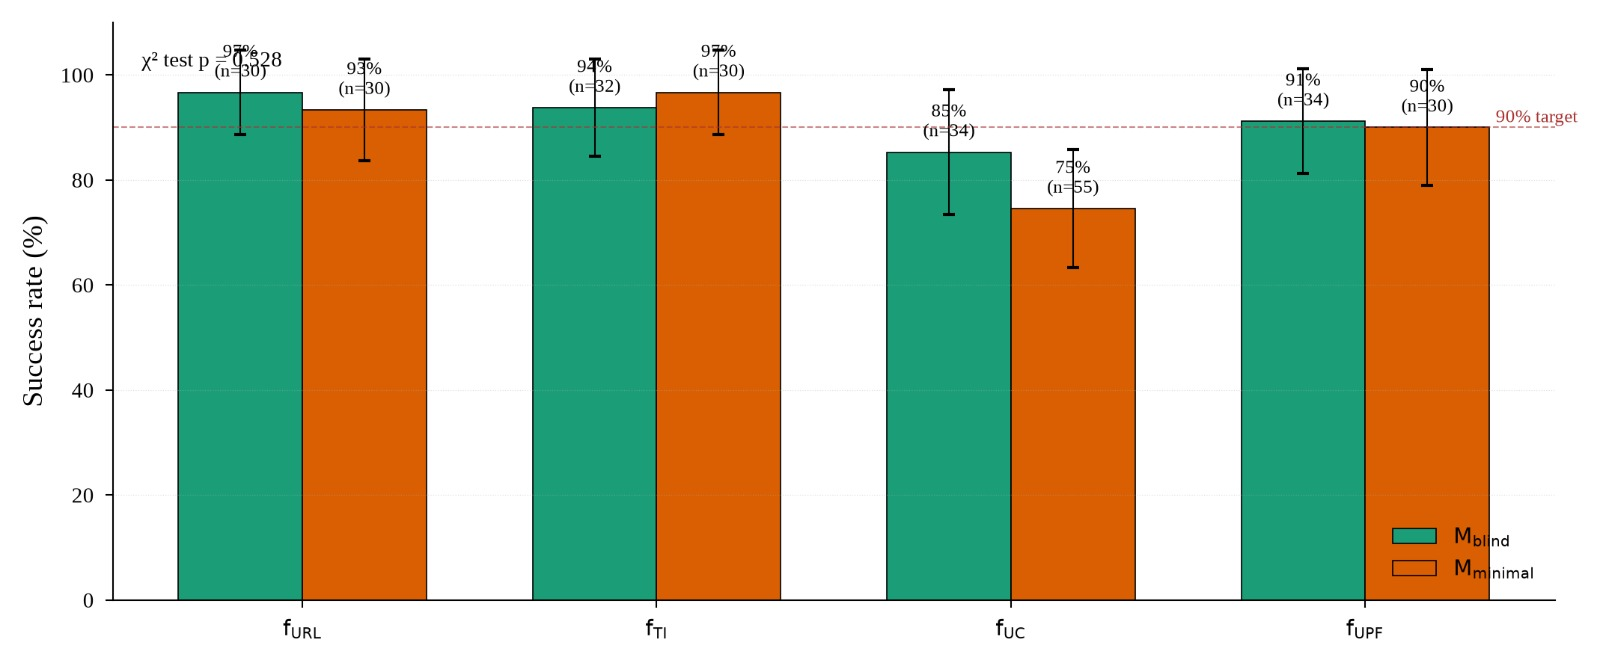
\includegraphics[width=0.5\linewidth]{Fig 5.jpeg}
    \caption{Recovery Success Rate by Fault Type and Method}
    \label{fig:placeholder}
\end{figure}

Both methods meet or come close to the 90\% target for most fault types. M\_blind reaches an overall success rate of 92.5\% (n=130), peaking at UE\_ROUTE\_LEAK (96.7\%, n=30). M\_minimal reaches 86.2\% overall (n=145), with its best result at TUNNEL\_INTERRUPTION (96.3\%, n=27). The lowest figure belongs to M\_minimal on UE\_CRASH (75.5\%, n=49), a drop traced back to the classifier confusing UE\_CRASH with UPF\_PATH\_FAILURE. A $X^2$ test gives p = 0.28, so the overall difference in success rate between the two methods is not statistically significant.

\subsection{Recovery Time Comparison}
Whether M\_minimal recovers faster than M\_blind is the focus here. Fig. 6 shows how recovery time is distributes for each fault type and method, with M\_minimal posting a 46\% lower median time overall (M\_blind pooled median $\sim$ 74s versus M\_minimal pooled median $\sim$ 20s; Mann-Whitney p $<$ 0.001, Cliff's $\delta$ = 0.977).

\begin{figure}
    \centering
    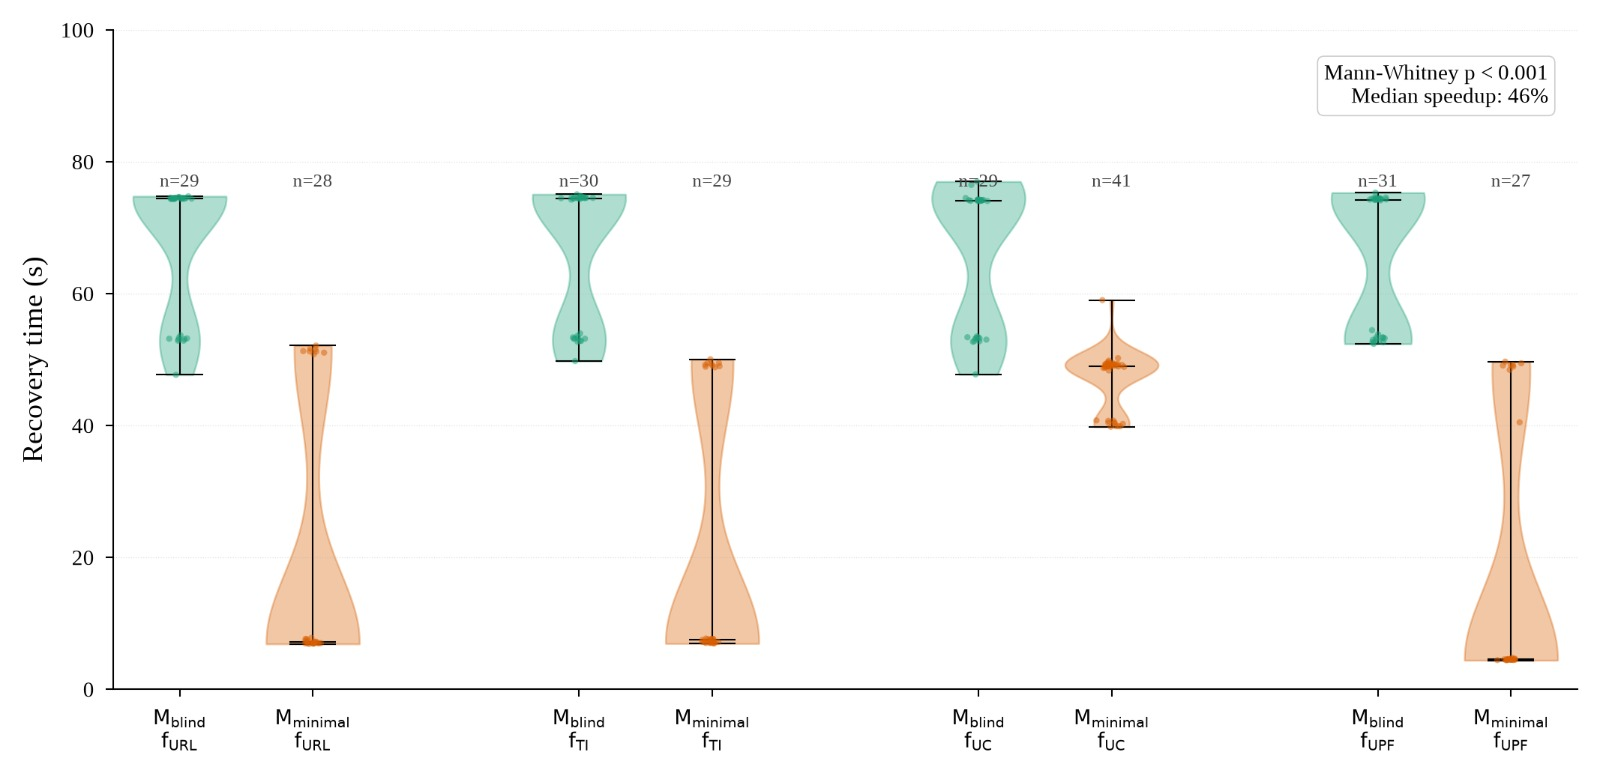
\includegraphics[width=0.5\linewidth]{Fig 6.jpeg}
    \caption{Recovery Time Distribution by Fault and Method}
    \label{fig:placeholder}
\end{figure}

M\_minimal finishes recovery faster across every fault category. For UE\_ROUTE\_LEAK and TUNNEL\_INTERRUPTION, it takes roughly 7-22 seconds, against 67-75 seconds for M\_blind. UE\_CRASH and UPF\_PATH\_FAILURE shows wider spread under M\_minimal because of occasional escalation, yet most runs still finish ahead of M\_blind. Pooling across fault types, M\_blind sits at a median of $\sim$ 74s while M\_minimal sits at approximately 20~s, a 46\% speedup (Mann-Whitney p $<$ 0.001, Cliff's $\delta$ = 0.977).

Fig.7 gives the empirical cumulative distribution of recovery time across fault types, which further illustrates how much faster M\_minimal recovers compared with M\_blind.

\begin{figure}
    \centering
    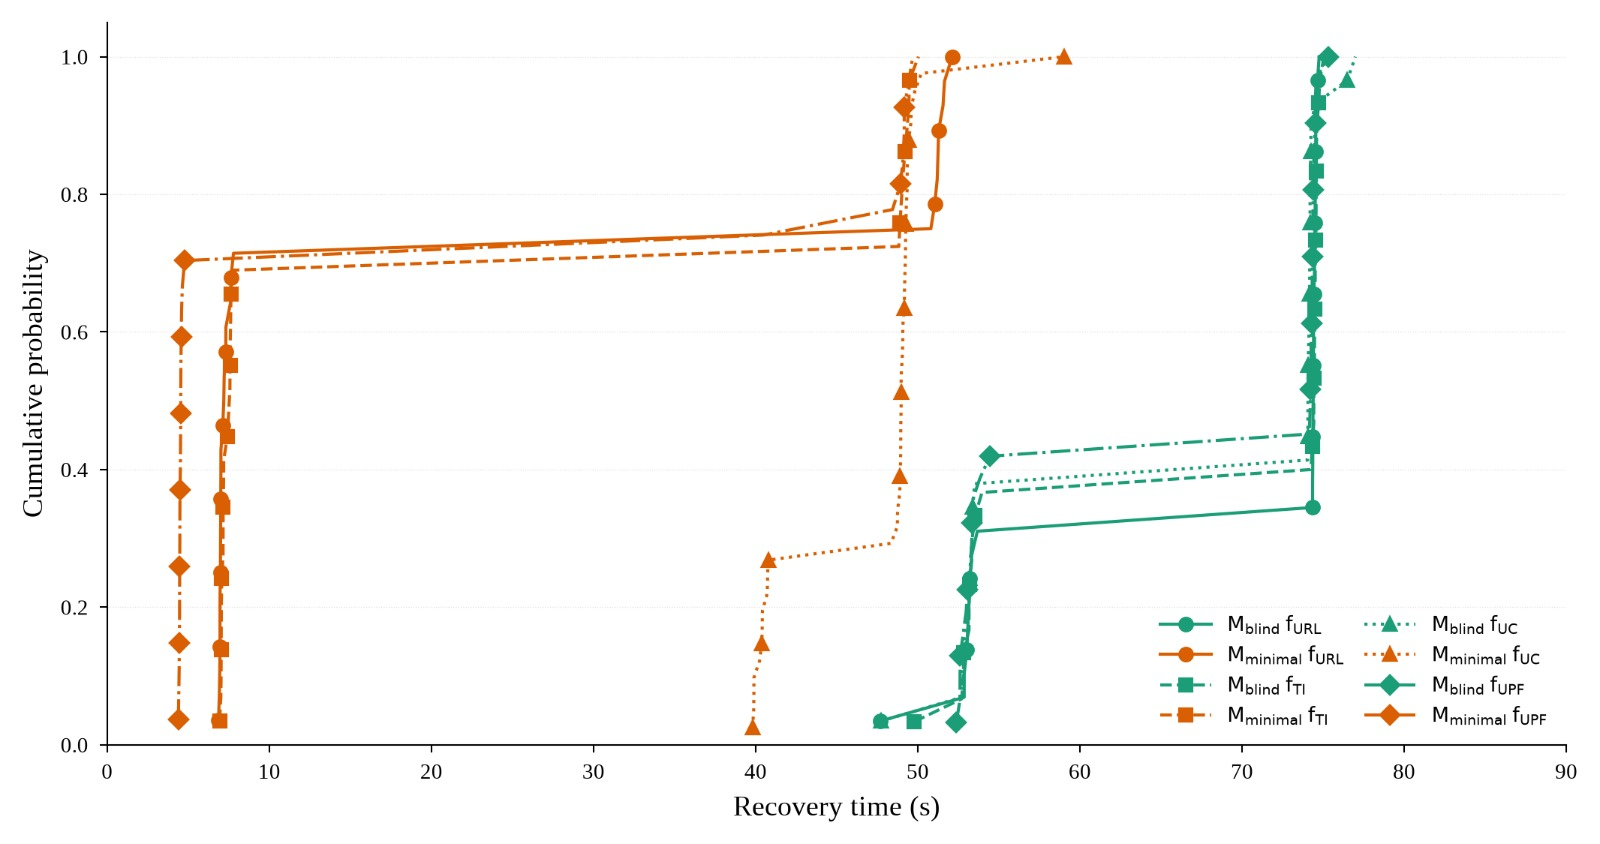
\includegraphics[width=0.5\linewidth]{Fig 7.jpeg}
    \caption{Emirical CDF of Recovery Time for M\_blind and M\_minimal Across Fault Types}
    \label{fig:placeholder}
\end{figure}

The CDF reveals two distinct clusters for M\_minimal: roughl;y 70\% of runs finish at 5-8s through single-action recovery, while the remaining approximately 30\% sit at 47-52s after escalating to fix\_ran\_userplan. M\_blind, by contrast, form a single cluster at 47-78s across all fault types. The gap between the M\_minimal (teal) and M\_minimal (orange) curves holds steady across every fault category, reinforcing the time advantage of the evidence-driven approach.

\subsection{Recovery Action Count Comparison}
Whether M\_minimal requires fewer recovery actions than  M\_minimal is examined here. Fig. 8 reports the mean number of actions per recovery and their composition for each fault type; M\_minimal needs fewer actions than M\_blind in every case (Mann-Whitney p $<$ 0.001).

\begin{figure}
    \centering
    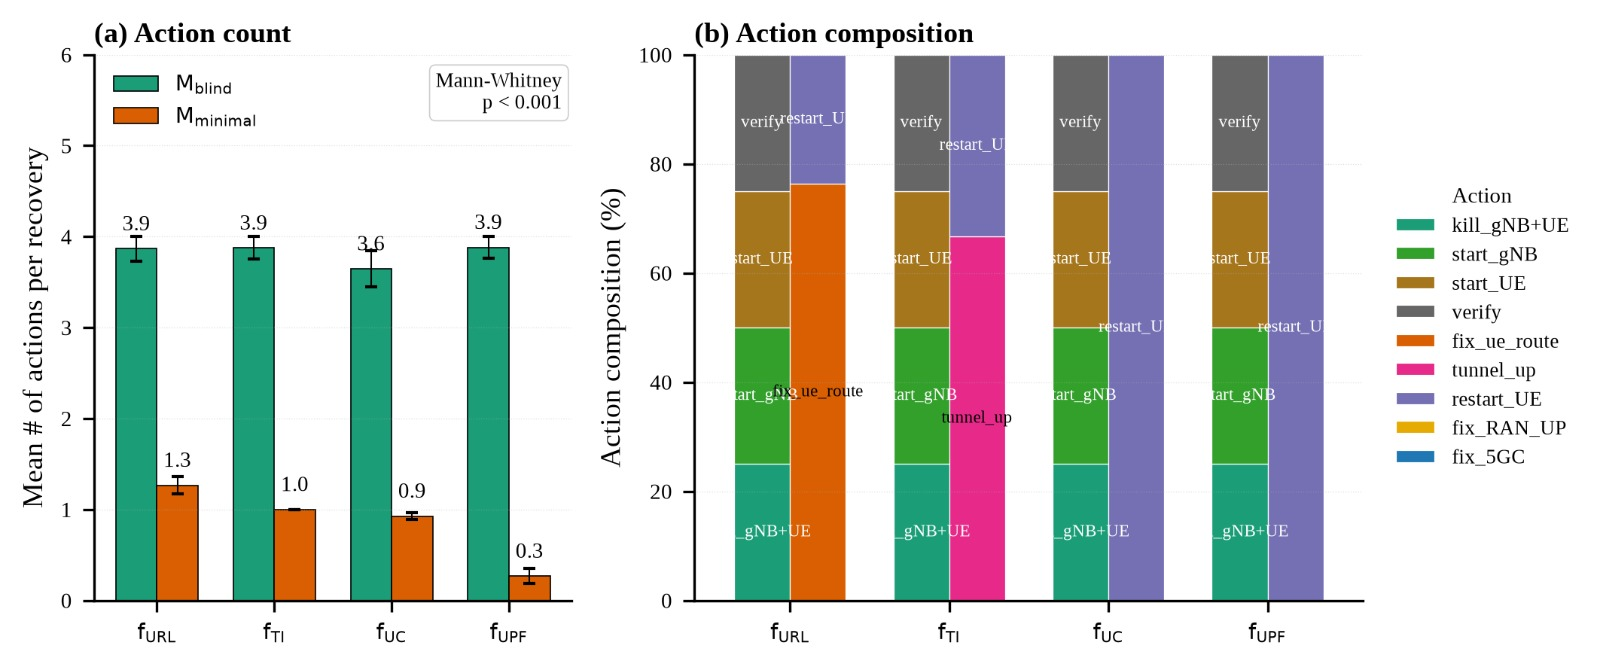
\includegraphics[width=0.5\linewidth]{Fig 8.jpeg}
    \caption{Recovery Action Count and Composition by Fault and Method}
    \label{fig:placeholder}
\end{figure}

M\_blind runs through roughly 4 action per recovery no matter the fault, since its restart sequence (kill\_gNB, start\_gNB, start\_UE, verify) is fixed. M\_minimal cuts this down sharply, averaging between 0.3 actions (UPF\_PATH\_FAILURE) and 1.3 actions (UE\_ROUTE\_LEAK) per run, since only the single action matched to the classified fault is fired. Where escalation kicks in (around 30\% of runs), the count rises to 2-3. This pattern reflect the contrast between M\_minimal's targeted, minimal interventions and M\_blind's blanket restart.

\subsection{Repeatability and Evidence Completeness}
Stability of recovery outcomes across repeated runs of the same fault scenario is the focus here. Fig. 9 plots the number of artifact files per run folder, drawn from an audit of 523 run folders covering all 275 CSV runs plus rerun and duplicate folders, and points to a statically significant gap in artifact counts between the methods (KS test p $<$ 0.001).

\begin{figure}
    \centering
    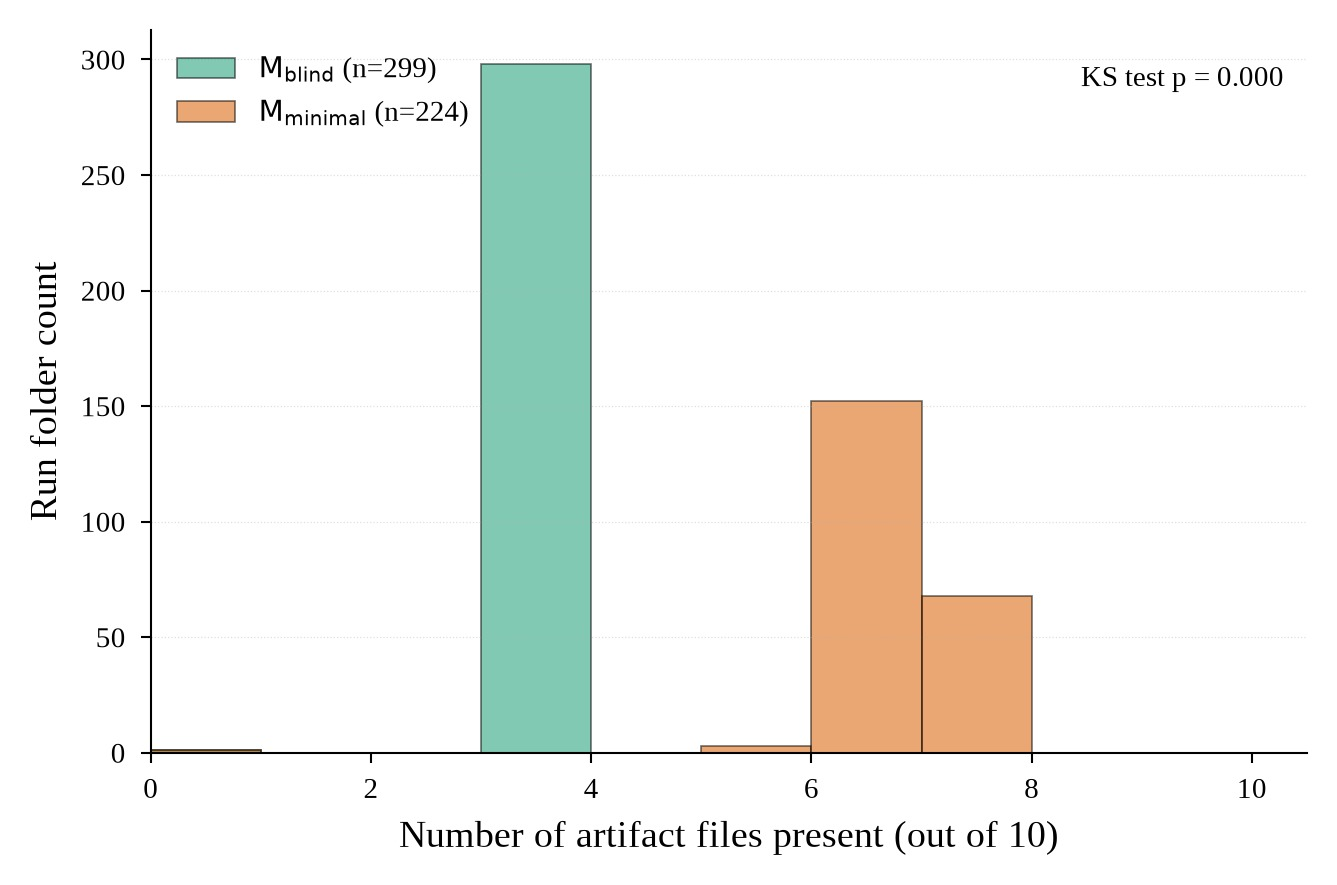
\includegraphics[width=0.5\linewidth]{Fig 9.jpeg}
    \caption{Distribution of Artifact File per Run Folder for M\_blind and M\_minimal}
    \label{fig:placeholder}
\end{figure}

M\_blind  folders hold 4 artifact file every time, while M\_minimal folders hold 6-8. reflecting the extra classification and evidence records the evidence-driven approach generates. This difference is statistically significant (KS test p $<$ 0.001), and the audit trail confirms that both methods leave complete, machine-readable records suitable for post-failure analysis and for reproducing the experiment.

\subsection{Sub-Sample Robustness Analysis}

Because M\_blind (n=130) and M\_minimal (n=145) ended up with unequal sample sizes, a balanced sub-sample of 130 runs per methods (260 runs total, seed=42) was drwan from the full 275 run dataset to check wheter this imbalance affected the conclusions.

The balanced results closely track the full datset: overall success rate comes out at 88.8\% versus 88.7\% for the full sample ($\Delta$ = 0.1 pp), and per-method rates stay unchanged (M\_blind 91.5\%, M\_minimal 86.2\%). M\_blind's sample size and success rate are identical in both datasets (n=130, SR=91.5\%), since the balancing procedure only trimmed M\_minimal runs. With a negligible effect size for success rate (Cliff's $\delta$ = 0.977), the main conclusions of this study hols up under sample-size imbalance and should generalize to balanced designs.

The same concerns about unequal method-level sample sizes  in the primary analysis (n = 275) was checked by re-running the comparisons on this balanced subsample (n = 260, 130 per method). Table 6 and 7  list the recomputed per-method statistics and the corresponding effect sizes alongside the balanced figures. Direction and magnitude are both preserved ($\Delta$$\delta$ $\leq$ 0.04 across all pairs), which indicates the main findings are not an artifact of sample-sizes imbalance.

Table 6. Balanced subsample analysis (n=260, 130 per method). Figures reflect the full sample (n = 272) after stratification to give equal representation across methods. The two leftmost columns five mean and standard deviation of the primary metric, while the two rightmost columns compare method-level distribution. The direction and size of the differences hold steady comparaed with the full smaple (n = 275), showing the main findings are not driven by sample-size imbalance across methods.

Table 7. Robustness of effect size under balanced subsampling (=260). Cliff's $\delta$ is computed on both the full sample (n = 275) and the balanced subsample (n = 260) for each pairwise comparason. Effects with |$\delta$| $\geq$ 0.147 are conventionally interpreted as non-negligible, and the near-identical $\delta$ values across both columns confirm that full-sample conclusions are not artifacts of unequal method representation. The largest shift ($\Delta$$\delta$ = 0.004) stays well inside the small-effect range, which supports the stability of the reported rankings.

Subsampling drew runs without replacement, stratified by method (seed = 42). Cliff's $\delta$ values are reported with 95\% confidence intervals, with the full numerical output available in subsample\_stats.txt (supplementary material).
The implication of these results, together with their placement within the broader literature on operational reliability and auto-recovery for OAI-based 5G testbed, are examined in the closing part of this pare.

\section{CONCLUSION}
\subsection{Conclusion}
An evidence-driven fault classification and minimal-first auto-recovery framework for OAI-based 5G SA/SNPN testbeds has been presented in this paper. The investigation finds that structured health monitoring, combined with multi-source evidence collection and a predefined fault taxonomy, can reliably replace ad-hoc, experience-dependent troubleshooting in open-source 5G laboratory environments.\\

The evidence-driven fault classifier reaches an overall (micro-weighted) accuracy of 87.5\% on a heald-out subset of n=16 classified runs (macro-averaged per-calss accuracy: 66.7\%), with perfect per-class accuracy for UE\_ROUTE\_LEAK and UE\_CRASH (100\% each), and primary ambiguity is the misclassification of both tunnel-related (TUNNEL\_INTERRUPTION, 33,3\%) and user-plane (UPF\_PATH\_FAILIRE), 100\%) faults toward the insfrastructure category (UE\_CRASH), owing to overlapping downstream escalation paths.

M\_minimal consistently outperforms M\_blind in recovery time across all four fault types, delivering a median speedup of 46\% (Mann-Whitney p $<$ 0.001, Cliff's $\delta$ = 0.977) and reducing the mean number of corrective actions from approximately 4 to a median of 1 per recovery, with no statistically significant difference in overall success rate between the two methods (p = 0.28). Third, both methods produce consistent artifact counts accross 523 audited run folders, condfirming that the operational workflow yields machine-readable records that support post-failure analysis and expereiment reporducibility.

Evidence-driven, minimal-first recovery thus offers a concrete and reproducible alternative to ad-hoc troubleshooting in opern-source 5G laboratotrty environments.\\

\subsection{Future Work}
Several questions opened by this wortk warrant further investigation. Future work needs to establish whether the fault classifier can be extended with machine-learning techniques to resolve ambiguity between overlapping fault categories -- particularly the UE\_CRASH and UPF\_PATH\_FAILURE classes -- and to assess the scalability of the framework to multi-node and multi-tenant O-RAN deployments. Additionally, integration with Near-RT RIC xApps and AI-assisted network control loops represents a promising direction for advancing toward full autonomous 5G network operations.


\section*{Acknowledgment}

The preferred spelling of the word ``acknowledgment'' in America is without 
an ``e'' after the ``g''. Avoid the stilted expression ``one of us (R. B. 
G.) thanks $\ldots$''. Instead, try ``R. B. G. thanks$\ldots$''. Put sponsor 
acknowledgments in the unnumbered footnote on the first page.

\section*{References}

Please number citations consecutively within brackets \cite{b1}. The 
sentence punctuation follows the bracket \cite{b2}. Refer simply to the reference 
number, as in \cite{b3}---do not use ``Ref. \cite{b3}'' or ``reference \cite{b3}'' except at 
the beginning of a sentence: ``Reference \cite{b3} was the first $\ldots$''

Number footnotes separately in superscripts. Place the actual footnote at 
the bottom of the column in which it was cited. Do not put footnotes in the 
abstract or reference list. Use letters for table footnotes.

Unless there are six authors or more give all authors' names; do not use 
``et al.''. Papers that have not been published, even if they have been 
submitted for publication, should be cited as ``unpublished'' \cite{b4}. Papers 
that have been accepted for publication should be cited as ``in press'' \cite{b5}. 
Capitalize only the first word in a paper title, except for proper nouns and 
element symbols.

For papers published in translation journals, please give the English 
citation first, followed by the original foreign-language citation \cite{b6}.

\begin{thebibliography}{00}
\bibitem{b1} G. Eason, B. Noble, and I. N. Sneddon, ``On certain integrals of Lipschitz-Hankel type involving products of Bessel functions,'' Phil. Trans. Roy. Soc. London, vol. A247, pp. 529--551, April 1955.
\bibitem{b2} J. Clerk Maxwell, A Treatise on Electricity and Magnetism, 3rd ed., vol. 2. Oxford: Clarendon, 1892, pp.68--73.
\bibitem{b3} I. S. Jacobs and C. P. Bean, ``Fine particles, thin films and exchange anisotropy,'' in Magnetism, vol. III, G. T. Rado and H. Suhl, Eds. New York: Academic, 1963, pp. 271--350.
\bibitem{b4} K. Elissa, ``Title of paper if known,'' unpublished.
\bibitem{b5} R. Nicole, ``Title of paper with only first word capitalized,'' J. Name Stand. Abbrev., in press.
\bibitem{b6} Y. Yorozu, M. Hirano, K. Oka, and Y. Tagawa, ``Electron spectroscopy studies on magneto-optical media and plastic substrate interface,'' IEEE Transl. J. Magn. Japan, vol. 2, pp. 740--741, August 1987 [Digests 9th Annual Conf. Magnetics Japan, p. 301, 1982].
\bibitem{b7} M. Young, The Technical Writer's Handbook. Mill Valley, CA: University Science, 1989.
\bibitem{b8} D. P. Kingma and M. Welling, ``Auto-encoding variational Bayes,'' 2013, arXiv:1312.6114. [Online]. Available: https://arxiv.org/abs/1312.6114
\bibitem{b9} S. Liu, ``Wi-Fi Energy Detection Testbed (12MTC),'' 2023, gitHub repository. [Online]. Available: https://github.com/liustone99/Wi-Fi-Energy-Detection-Testbed-12MTC
\bibitem{b10} ``Treatment episode data set: discharges (TEDS-D): concatenated, 2006 to 2009.'' U.S. Department of Health and Human Services, Substance Abuse and Mental Health Services Administration, Office of Applied Studies, August, 2013, DOI:10.3886/ICPSR30122.v2
\bibitem{b11} K. Eves and J. Valasek, ``Adaptive control for singularly perturbed systems examples,'' Code Ocean, Aug. 2023. [Online]. Available: https://codeocean.com/capsule/4989235/tree
\end{thebibliography}

\vspace{12pt}
\color{red}
IEEE conference templates contain guidance text for composing and formatting conference papers. Please ensure that all template text is removed from your conference paper prior to submission to the conference. Failure to remove the template text from your paper may result in your paper not being published.

\end{document}
